\section{model+X}
\subsection{BP神经网络+X}
在I64,I96,I128上进行SVM的分类结果如图~\ref{table:bpx1}
\begin{table}[htb]
\centering
\caption{SVM在I64,I96,I128上的分类结果准确率}
\begin{tabular}{ccccc}
\toprule[2pt]
数据集 & svm,linear & svm,poly & svm,rbf & svm,sigmoid \\ 
I64 & 0.361199 & 0.524569 & 0.486280 & 0.081685 \\ 
I96 & 0.388641 & 0.534142 & 0.507339 & 0.086790 \\ 
I128 & 0.373325 & 0.559668 & 0.507977 & 0.356733 \\ 
\bottomrule[2pt]
\end{tabular}
\label{table:bpx1}
\end{table} 

首先考虑在BP神经网络系列实验中选取4个准确率较高的模型,分别用BP-A,BP-B,BP-C,BP-D进行编号,具体情况如表~\ref{table:bpx2}
\begin{table}[htb]
\centering
\caption{BP-A,BP-B,BP-C,BP-D模型概况}
\begin{tabular}{ccccc}
\toprule[2pt]
model & BP-A & BP-B & BP-C & BP-D \\ 
\midrule[1pt]
隐含层 & 1000 & 1000 & 500 & 500 \\ 
所用数据集 & I64 & I96 & I96 & I96 \\ 
学习率 & 0.03 & 0.03 & 0.03 & 0.03 \\ 
优化函数 & MGD & MGD & MGD & MGD \\ 
正则化参数 & 0 & 0 & 0 & 0.0001 \\ 
\midrule[1pt]
准确率 & 0.518188 & 0.522655 & 0.516273 & 0.49649 \\ 
\bottomrule[2pt]
\end{tabular} 
\label{table:bpx2}
\end{table}

由于SVM在分类问题上取得很好的效果,考虑将softmax换成SVM,有~\ref{table:bpx3}
\begin{table}[htb]
\centering
\caption{第一列为原始的BP-A,BP-B,BP-C,BP-D准确率,第二列为svm在I64,I96上的准确率,第三到第六列为BP-A,BP-B,BP-C,BP-D中将softmax层换成SVM,并依次选取linear,poly,rbf,sigmoid核后的准确率}
\begin{tabular}{ccccccc}
\toprule[2pt]
\ &softmax &svm-poly &nsvm-linear & nsvm-poly & nsvm-rbf & nsvm-sigmoid \\ 
BP-A & 0.518188 & 0.524569 & 0.538609 & 0.576260 & 0.587109 & 0.081685 \\ 
BP-B & 0.522655 & 0.534142 & 0.530951 & 0.577537 & 0.590938 & 0.075303 \\ 
BP-C & 0.516273 & 0.534142 & 0.507339 & 0.541799 & 0.580728 & 0.066369 \\ 
BP-D & 0.49649 & 0.534142 & 0.529675 & 0.572431 & 0.594129 & 0.356733 \\ 
\bottomrule[2pt]
\end{tabular} 
\label{table:bpx3}
\end{table}

为了更为直观展现结果,上表对应的条形图~\ref{fig:bpx1}如下
\begin{figure}[htb]
\centering
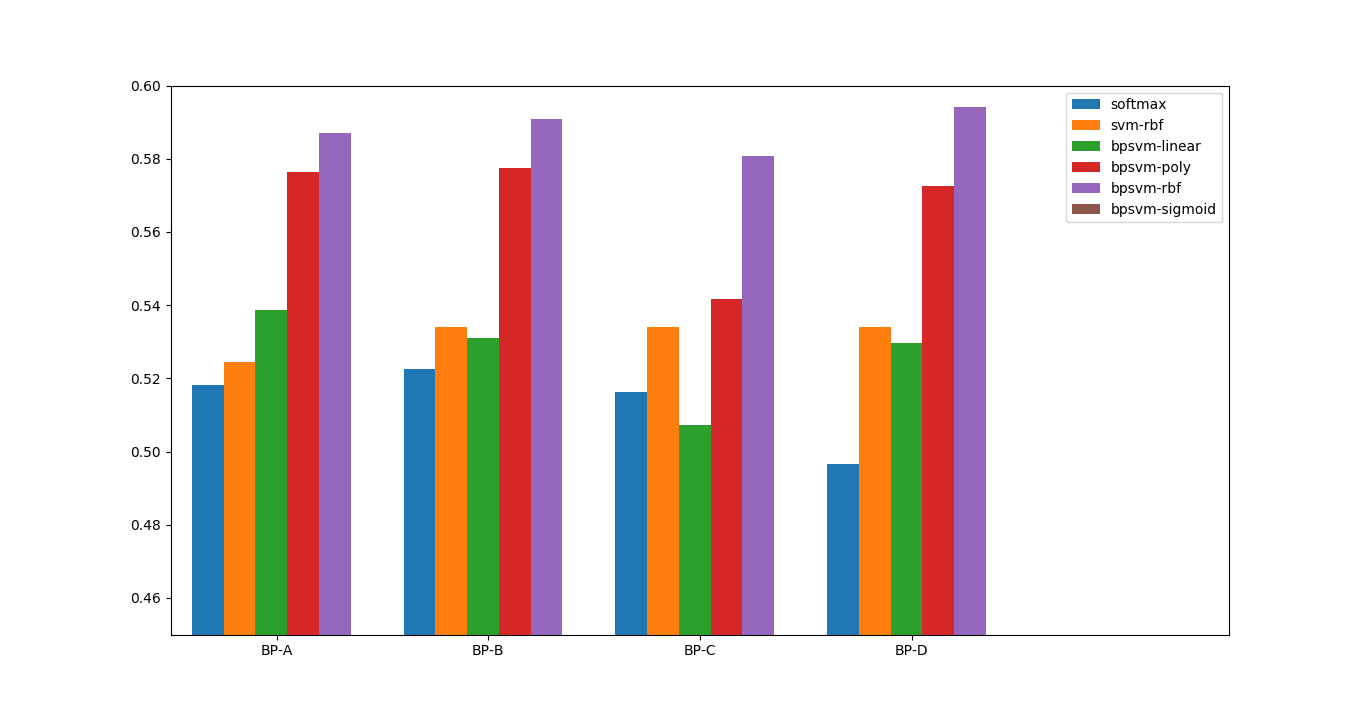
\includegraphics[scale=0.5]{../figures/NN_svm1.png} 
\caption{原始的BP-A,BP-B,BP-C,BP-D,SVM,与用SVM替换BP-A,BP-B,BP-C,BP-D中softmax层所得的准确率图}
\label{fig:bpx1}
\end{figure}

尝试使用决策树代替softmax,与SVM进行对比,有~\ref{table:bpx4}
\begin{table}[htb]
\centering
\caption{第1列为原始的BP-A,BP-B,BP-C,BP-D准确率,第2列为nsvm-rbf准确率,第3到6列为用CART树代替softmax的准确率,其中mdh代表最大深度。}
\begin{tabular}{cccccccc}
\toprule[2pt]
model  & softmax & nsvm-rbf & nCART-mdh:5 & nCART-mdh:10 & nCART-mdh:15 & nCART-mdh:20\\ 
A & 0.518188 & 0.587109 & 0.414167 & 0.417358 & 0.408424 & 0.411615\\ 
B & 0.522655 & 0.590938 & 0.416720 & 0.398851 & 0.387364 & 0.391078\\ 
C & 0.516273 & 0.580728 & 0.353542 & 0.337588 & 0.325463 & 0.327378\\ 
D & 0.49649 & 0.594129 & 0.395662 & 0.398851 & 0.389917 & 0.391193\\ 
\bottomrule[2pt]
\end{tabular} 
\label{table:bpx4}
\end{table}


为了更为直观展现结果,上表对应的条形图~\ref{fig:bpx2}如下
\begin{figure}[htb]
\centering
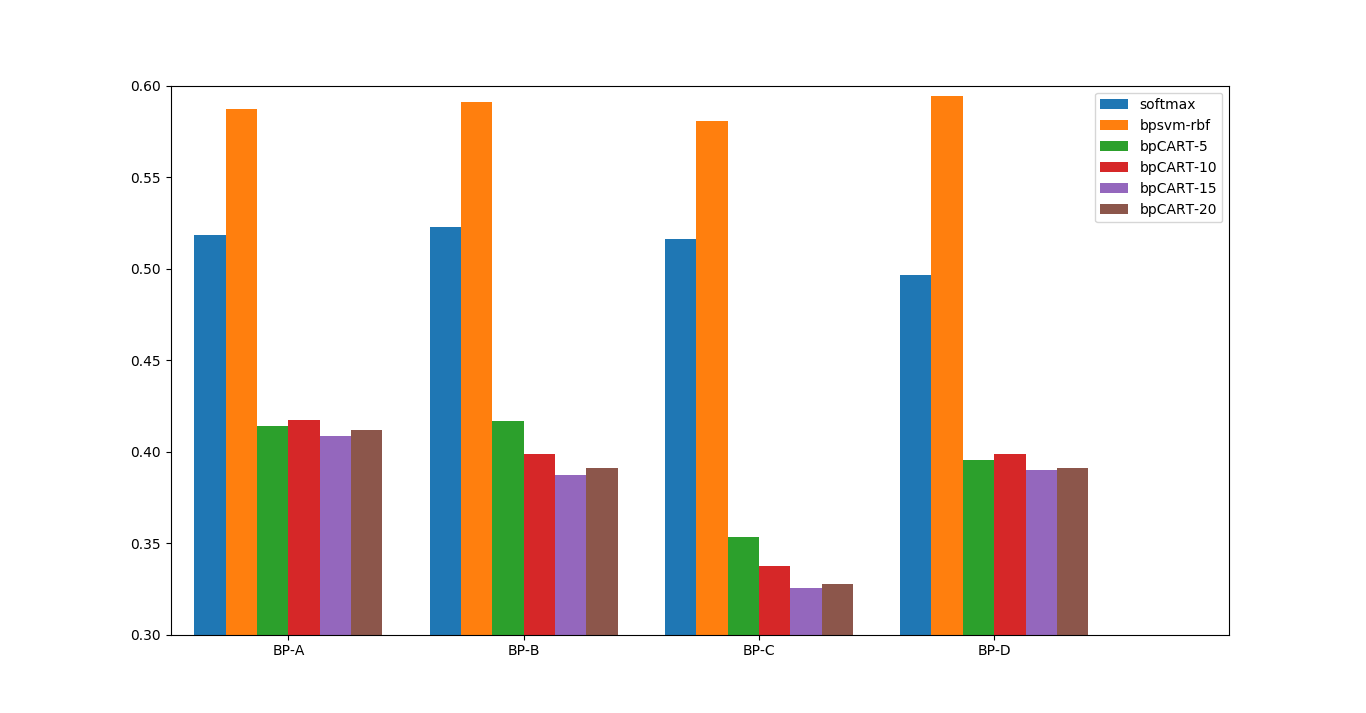
\includegraphics[scale=0.5]{../figures/NN_tree1.png} \\
\caption{原始的BP-A,BP-B,BP-C,BP-D,nsvm-rbf,与用不同深度的CART替换softmax层所得的准确率图}
\label{fig:bpx2}
\end{figure}


尝试使用随机森林代替softmax,与SVM进行对比,结果如~\ref{table:bpx5}

\begin{table}[htb]
\centering
\caption{第1列为原始的BP-A,BP-B,BP-C,BP-D准确率,第2列为nsvm-rbf准确率,第3到6列为用随机森林代替softmax的准确率,其中,n代表随机森林包含的树桩个数。}
\begin{tabular}{cccccc}
\toprule[2pt]
model & softmax & nsvm,rbf & nrf-n:20 & nrf-n:50 & nrf-n:80 \\ 
A & 0.518188 & 0.587109 & 0.544352 & 0.552010 & 0.573070 \\ 
B & 0.522655 & 0.590938 & 0.530313 & 0.559668 & 0.574346 \\ 
C & 0.516273 & 0.5580728 & 0.504786 & 0.534780 & 0.555839 \\  
D & 0.49649 & 0.594129 & 0.523293 & 0.561583 & 0.555839 \\ 
\midrule[2pt]
model & nrf-n:110 & nrf-n:140 & nrf-n:170 & nrf-n:200 & nrf-n:230 \\ 
A & 0.574346 & 0.569879 & 0.577537 & 0.580089 & 0.574984 \\ 
B & 0.569879 & 0.586471 & 0.596043 & 0.583918 & 0.575622 \\ 
C & 0.545629 & 0.557754 & 0.550734 & 0.562221 & 0.569241 \\ 
D & 0.560944 & 0.573070 & 0.576899 & 0.580089 & 0.579451 \\ 
\bottomrule[2pt]
\end{tabular} 
\label{table:bpx5}
\end{table}


\begin{figure}[htb]
\centering
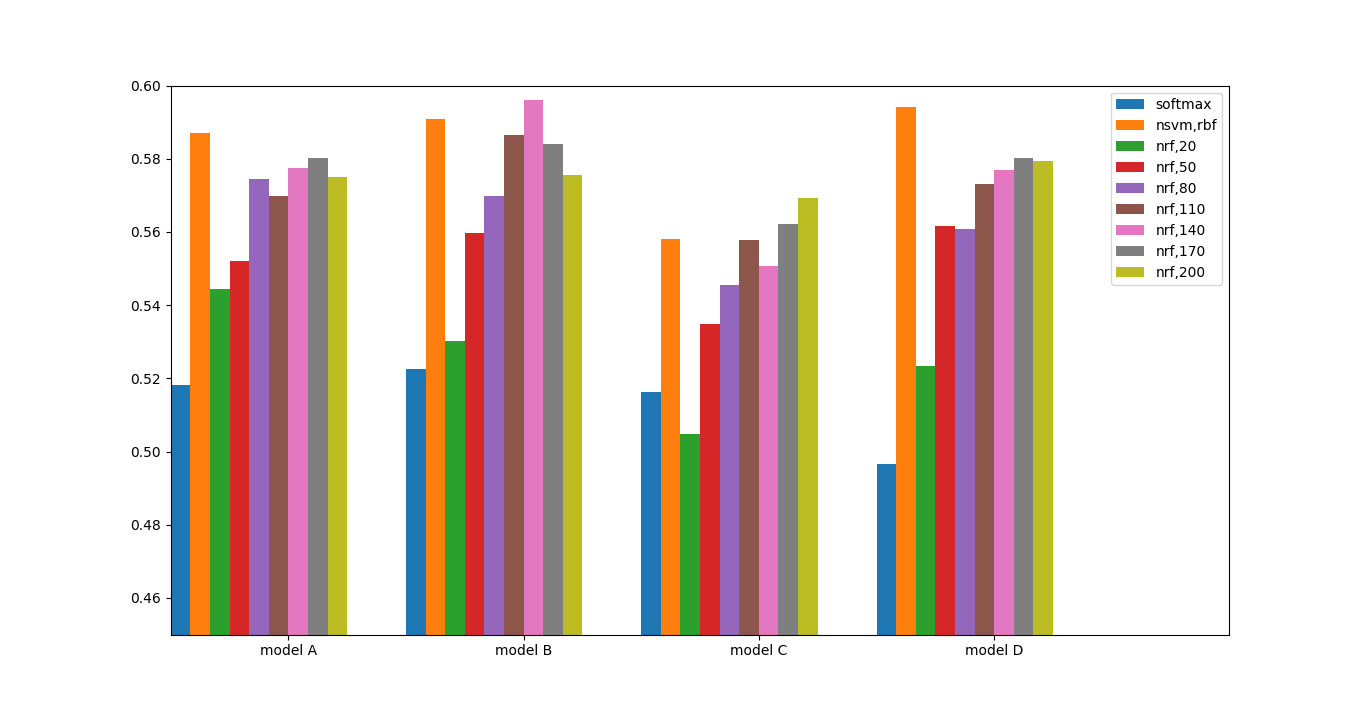
\includegraphics[scale=0.5]{../figures/NN_rf1.png} \\
\caption{原始的 BP-A,BP-B,BP-C,BP-D,nsvm-rbf,与用包含不同树桩个数的随机森林替softmax 层所得的准确率图}
\label{fig:bpx3}
\end{figure}


\subsection{CNN+X}
\begin{table}[htb]
\centering
\begin{tabular}{cccccc}
\toprule[2pt]
model & softmax & cnsvm,linear & cnsvm,poly & cnsvm,rbf & cnsvm,sigmoid \\ 
CNN-A & 0.652202 & 0.649649 & 0.654116 & 0.167837 & 0.110402\\ 
CNN-B & 0.664327 & 0.642629 & 0.701340 & 0.219528 & 0.084876\\ 
CNN-C & 0.673899 & 0.639438 & 0.693044 & 0.248883 & 0.156988\\ 
CNN-D & 0.659860 & 0.624123 & 0.682195 & 0.375877 & 0.127632\\ 
\bottomrule[2pt]
\end{tabular} 
\label{table:cnnx1}
\end{table}


\begin{center}
\begin{tabular}{cccccc}
\toprule[2pt] 
model & softmax  & cnsvm,poly & nrf,20 & nrf,50 & nrf,80 \\ 
E & 0.652202 & 0.654116 & 0.644544 & 0.662412 & 0.671985 \\ 
F & 0.664327 & 0.701340 & 0.611997 & 0.659221 & 0.647096 \\ 
G & 0.673899 & 0.693044 & 0.622846 & 0.663689 & 0.672623 \\ 
H & 0.659860 & 0.682195 & 0.624761 & 0.652840 & 0.668156 \\ 
\midrule[2pt]
model & nrf,110 & nrf,140 & nrf,170 & nrf,200 & nrf,230 \\ 
E & 0.677090 & 0.694320 & 0.700702 & 0.693044 & 0.703255 \\ 
F & 0.657945 & 0.661136 & 0.664327 & 0.675176 & 0.665603 \\  
G & 0.684110 & 0.673261 & 0.682195 & 0.677090 & 0.690491 \\ 
H & 0.669432 & 0.665603 & 0.677728 & 0.675176 & 0.686662 \\ 
\bottomrule[2pt]
\end{tabular} 
\end{center}


\begin{center}
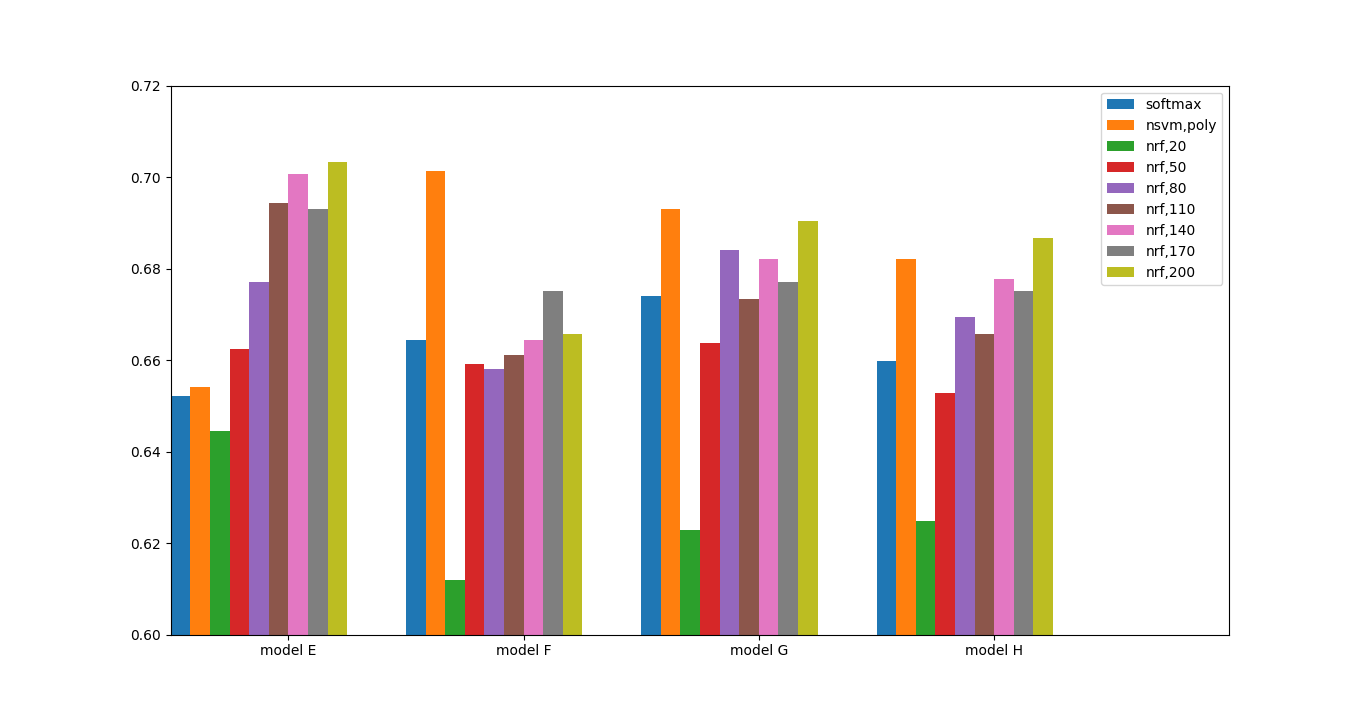
\includegraphics[scale=0.5]{../figures/CNN_rf1.png} \\
BP神经网络+CART。model A指$64\times64$,隐含层神经元个数为1000;model B指$96\times96$,隐含层神经元个数为1000;model C指$96\times96$,隐含层神经元个数为500;model D指$96\times96$,隐含层神经元个数为500,正则化系数为0.0001。
\end{center}
